\documentclass[11pt,letterpaper,final]{report}
\usepackage[utf8]{inputenc}
\usepackage[francais]{babel}
\usepackage[T1]{fontenc}
\usepackage{amsmath}
\usepackage{amsfonts}
\usepackage{amssymb}
\usepackage{graphicx}
\usepackage{lmodern}
\usepackage[left=2.54cm,right=2.54cm,top=2.54cm,bottom=2.54cm]{geometry}
\begin{document}
\chapter{Cross validation entre les différentes plateformes de simulations}
Dans ce chapitre, nous allons comparer les différents simulateurs par rapport à certains de leur paramètres observables lors des simulations. Les paramètres seront testé sur  7 simulations diférentes éparpillé sous deux catégories, des simulations se rapportant à la configuration NPC et d'autres par rapport au fonctionnement d'un hacheur. De plus, chaque simulateur sera testé à un pas de calcul de 1us, 5us et 50us.
\section{Pont DCP/DCN: Validation PSIM/SPS}
\subsection{Hacheur 4 quadrants}
\subsubsection{Vérification à un pas de calcul de 50us}


\begin{figure}[h!]
\centering
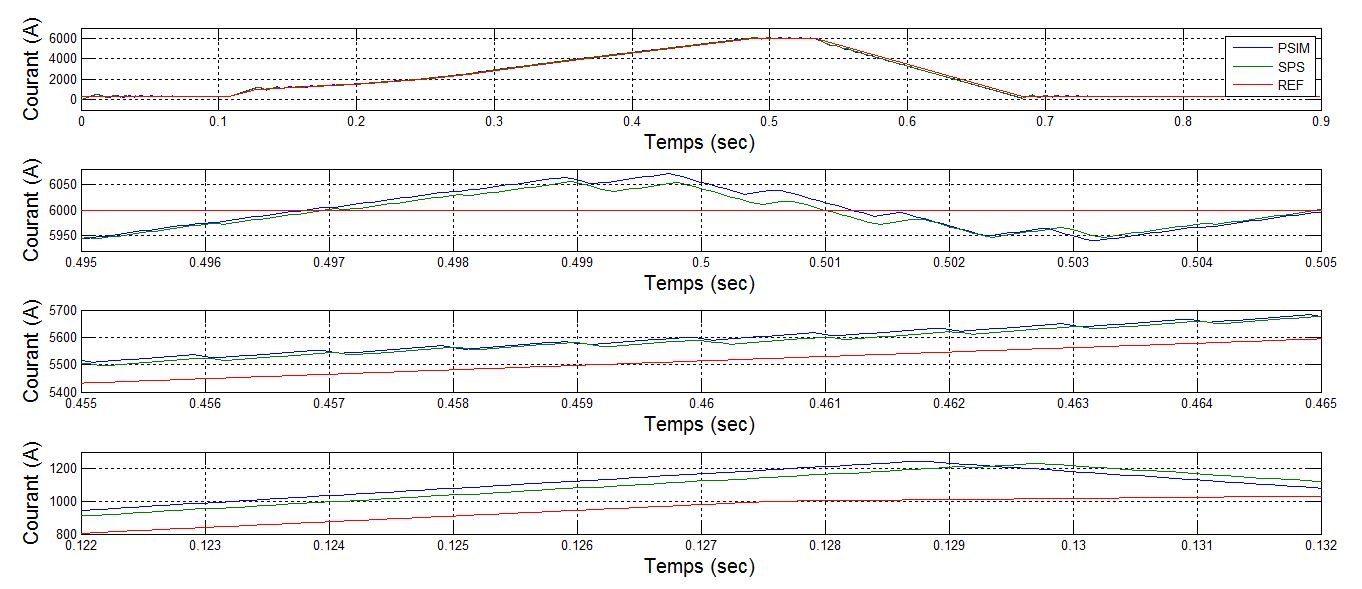
\includegraphics[scale=0.5]{Fig/Hacheur4Quadrants/HacheurCourantCharge50u.jpg}
\caption{Le courant sur la charge PSIM et SPS à un pas de calcul de 50us}
\label{comp_PSIM_SPS}
\end{figure}


\begin{figure}[h!]
\centering
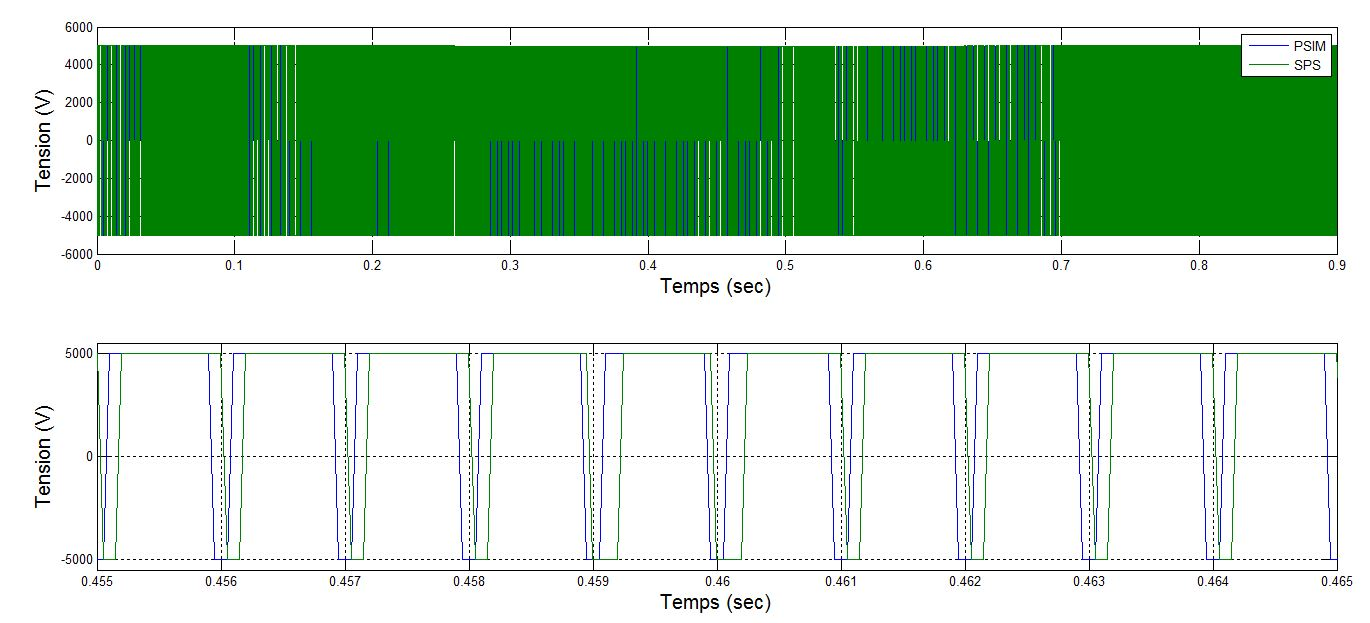
\includegraphics[scale=0.5]{Fig/Hacheur4Quadrants/HacheurTensionCharge50u.jpg}
\caption{La tension sur la charge PSIM et SPS à un pas de calcul de 50us}
\label{err_cou}
\end{figure}


\begin{figure}[h!]
\centering
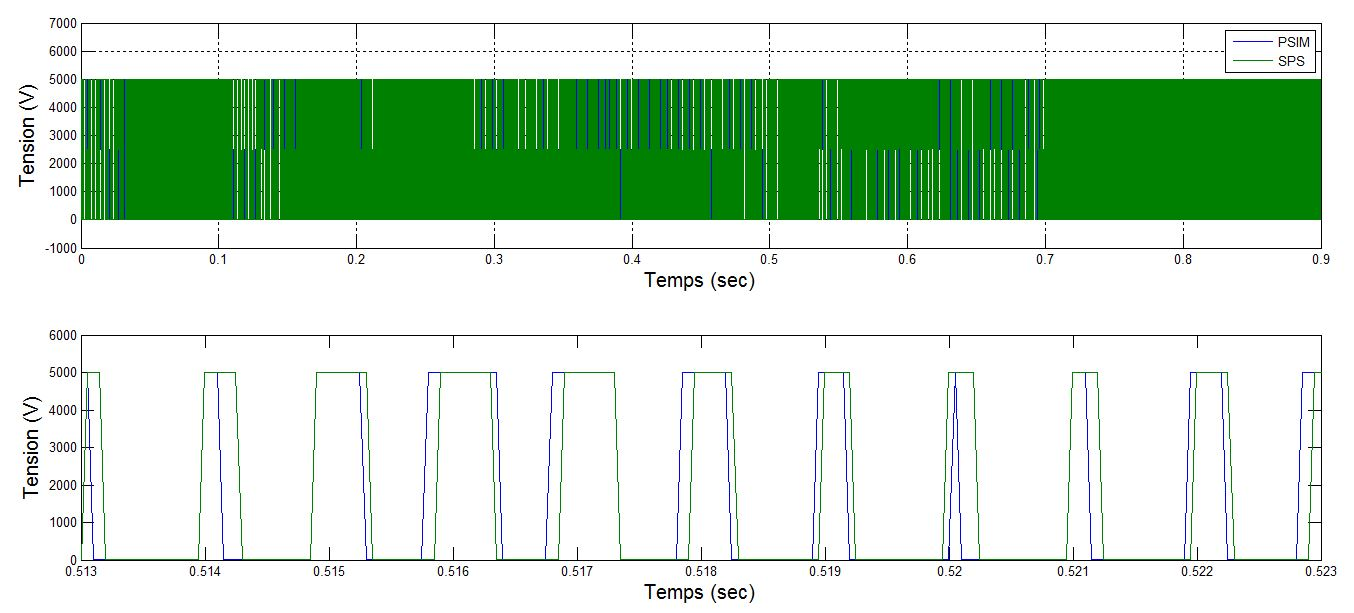
\includegraphics[scale=0.5]{Fig/Hacheur4Quadrants/HacheurTensionIGBT50u.jpg}
\caption{La tension au IGBT PSIM et SPS à un pas de calcul de 50us}
\label{hc_IG_ten_50}
\end{figure}

\begin{figure}[h!]
\centering
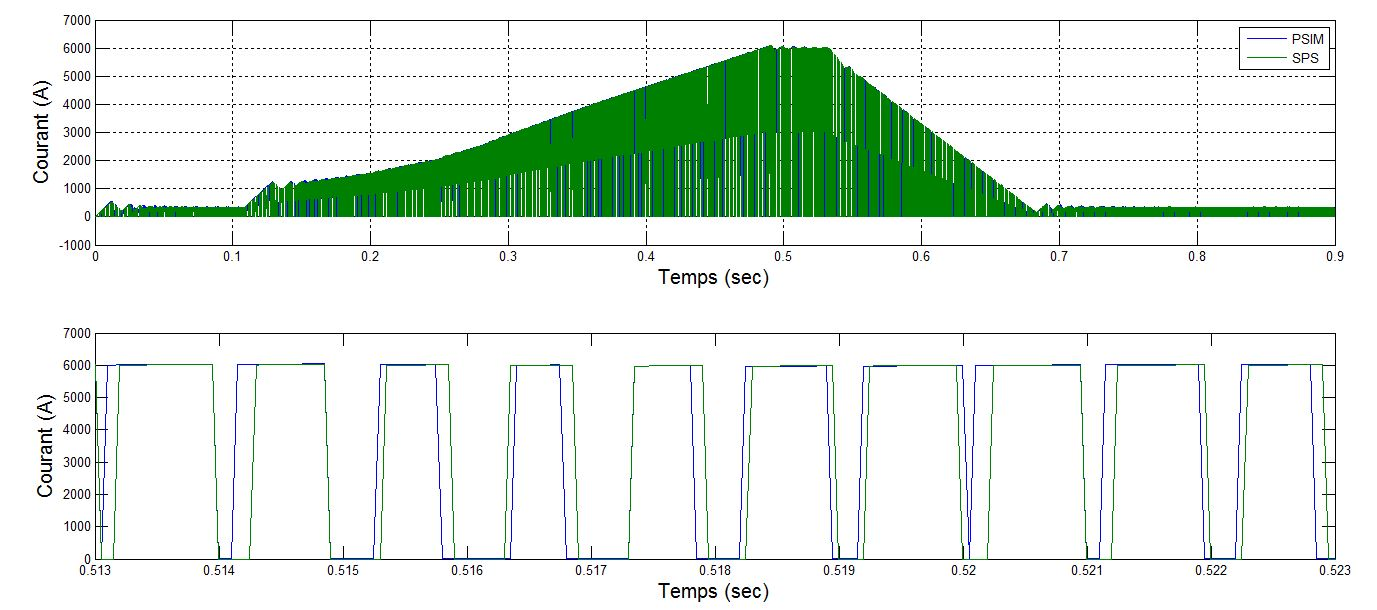
\includegraphics[scale=0.5]{Fig/Hacheur4Quadrants/HacheurCourantIGBT50u.jpg}
\caption{La tension au IGBT PSIM et SPS à un pas de calcul de 50us}
\label{hc_IG_cou_50}
\end{figure}
\clearpage
\subsubsection{Vérification à un pas de calcul de 5us}


\begin{figure}[h!]
\centering
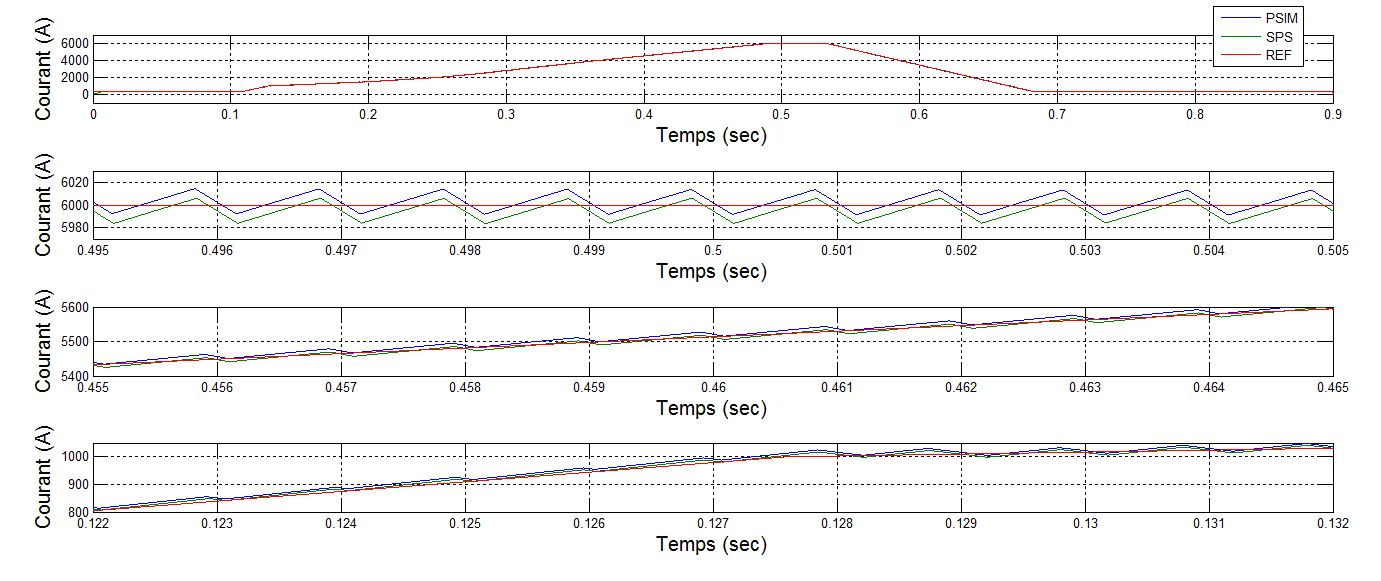
\includegraphics[scale=0.5]{Fig/Hacheur4Quadrants/HacheurCourantCharge5u.jpg}
\caption{Le courant sur la charge PSIM et SPS à un pas de calcul de 5us}
\label{hc_cou_ch_5}
\end{figure}


\begin{figure}[h!]
\centering
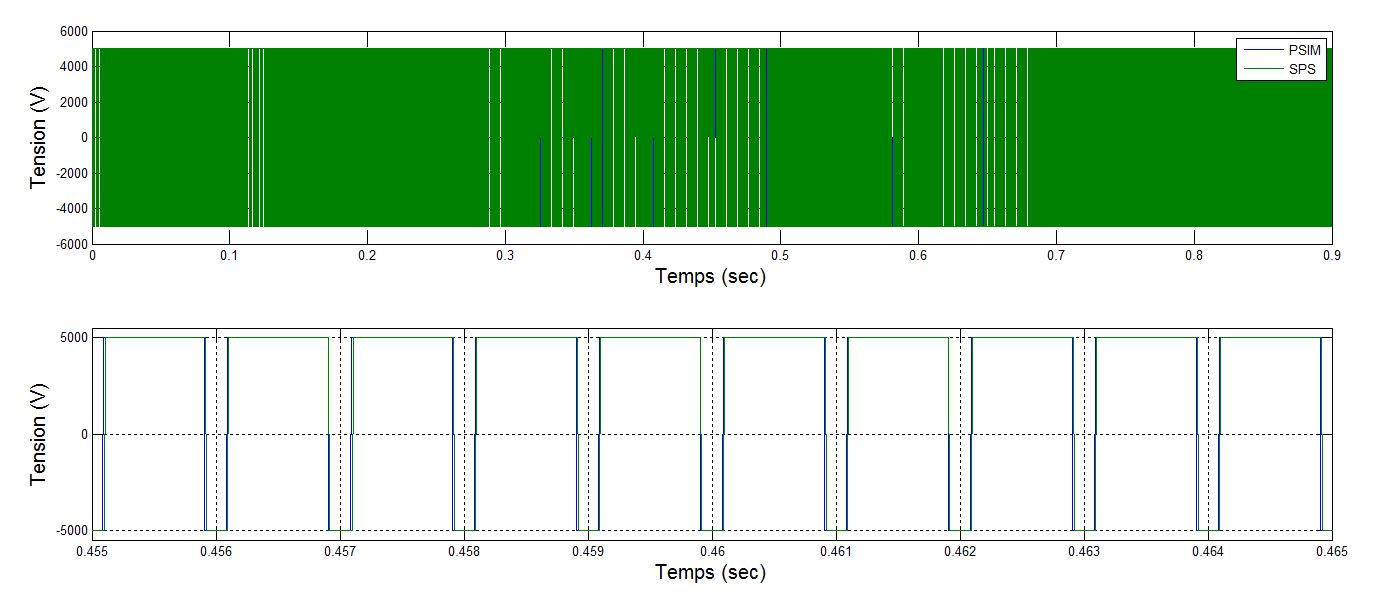
\includegraphics[scale=0.5]{Fig/Hacheur4Quadrants/HacheurTensionCharge5u.jpg}
\caption{La tension sur la charge PSIM et SPS à un pas de calcul de 5us}
\label{hc_ten_ch_5}
\end{figure}


\begin{figure}[h!]
\centering
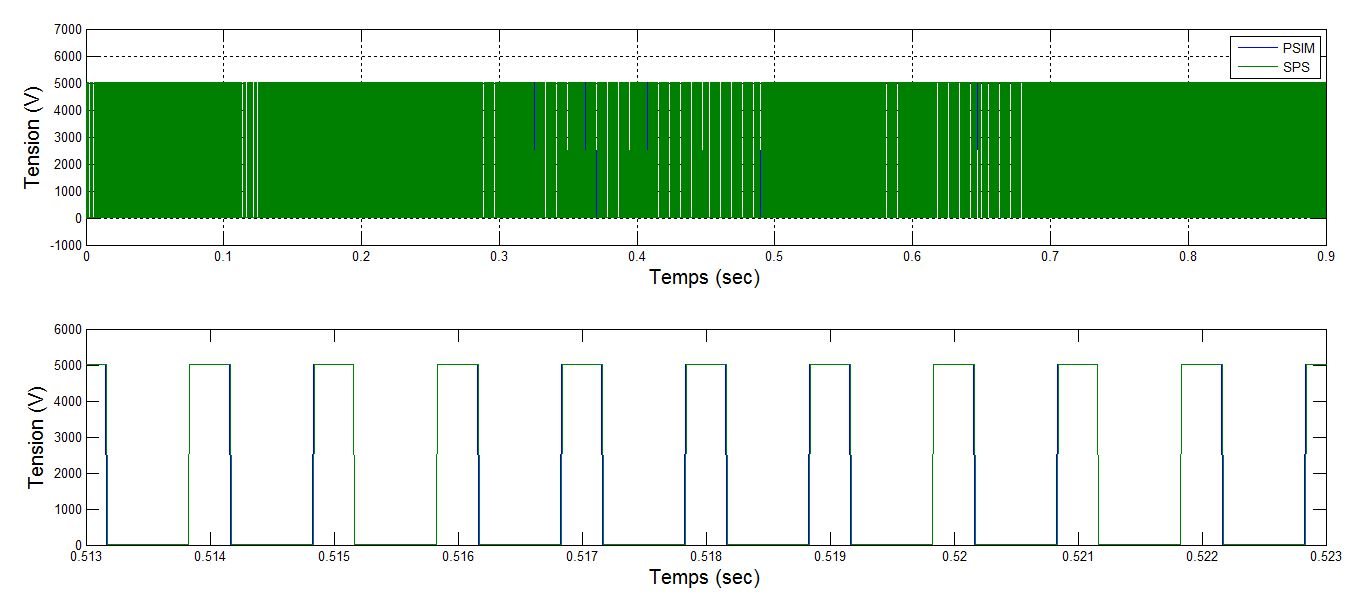
\includegraphics[scale=0.5]{Fig/Hacheur4Quadrants/HacheurTensionIGBT5u.jpg}
\caption{La tension au IGBT PSIM et SPS à un pas de calcul de 5us}
\label{hc_IG_ten_5}
\end{figure}

\begin{figure}[h!]
\centering
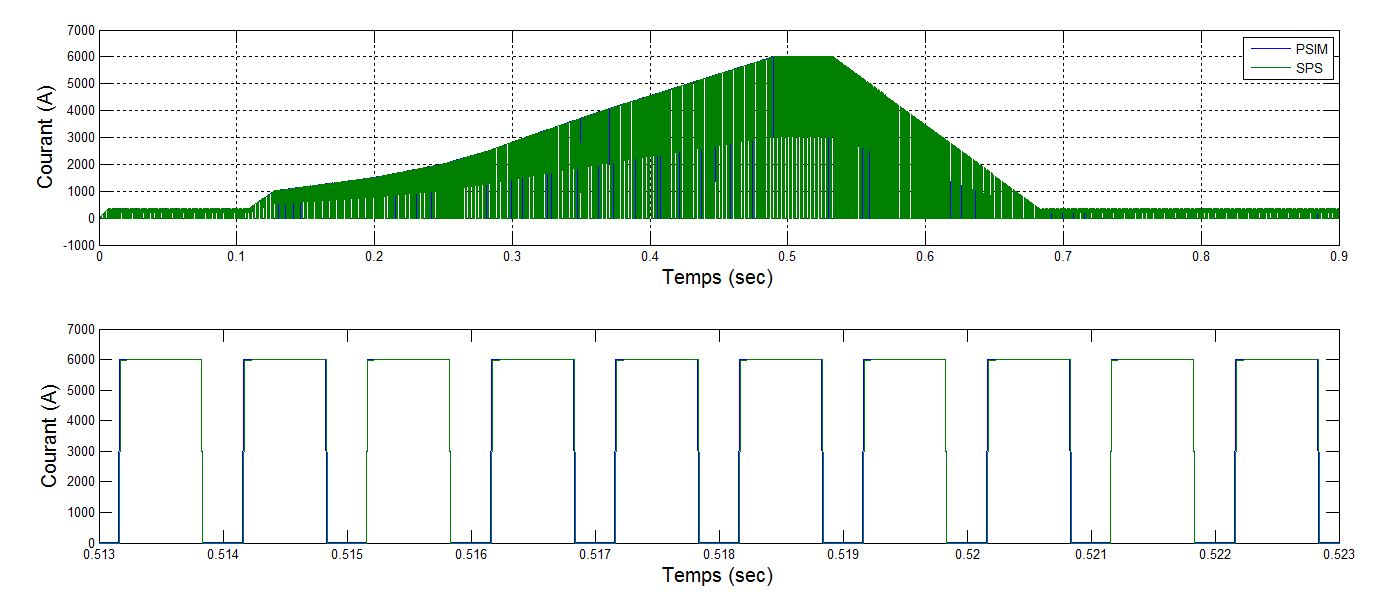
\includegraphics[scale=0.5]{Fig/Hacheur4Quadrants/HacheurCourantIGBT5u.jpg}
\caption{La tension au IGBT PSIM et SPS à un pas de calcul de 5us}
\label{hc_IG_cou_5}
\end{figure}
\clearpage
\subsubsection{Vérification à un pas de calcul de 1us}


\begin{figure}[h!]
\centering
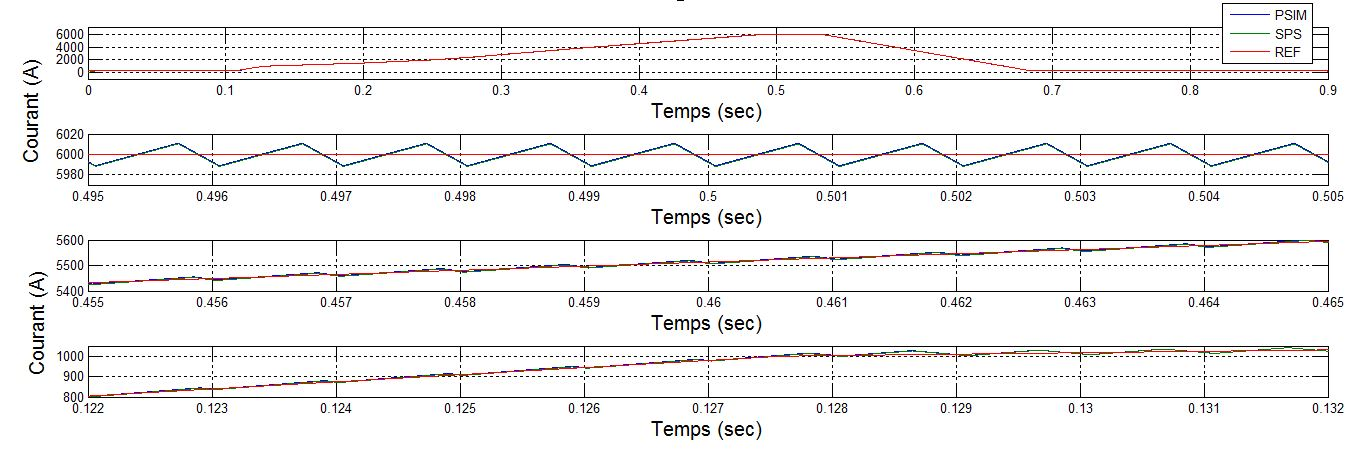
\includegraphics[scale=0.5]{Fig/Hacheur4Quadrants/HacheurCourantCharge1u.jpg}
\caption{Le courant sur la charge PSIM et SPS à un pas de calcul de 1us}
\label{hc_cou_ch_1}
\end{figure}


\begin{figure}[h!]
\centering
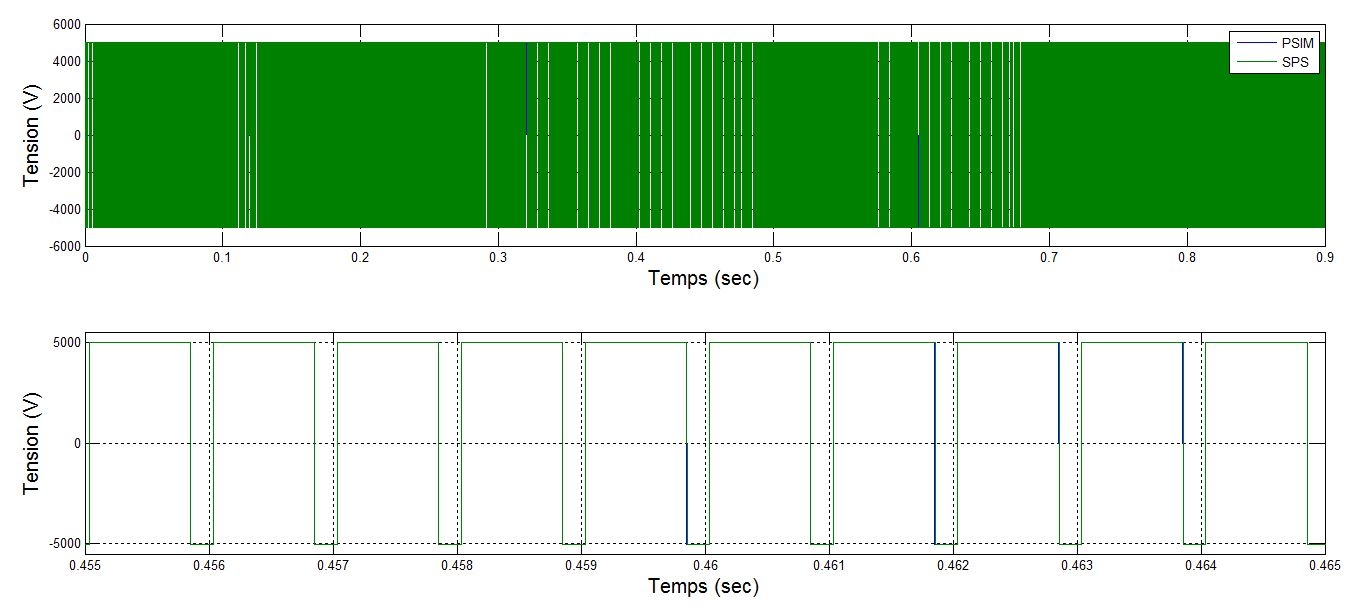
\includegraphics[scale=0.5]{Fig/Hacheur4Quadrants/HacheurTensionCharge1u.jpg}
\caption{La tension sur la charge PSIM et SPS à un pas de calcul de 1us}
\label{hc_ten_ch_1}
\end{figure}


\begin{figure}[h!]
\centering
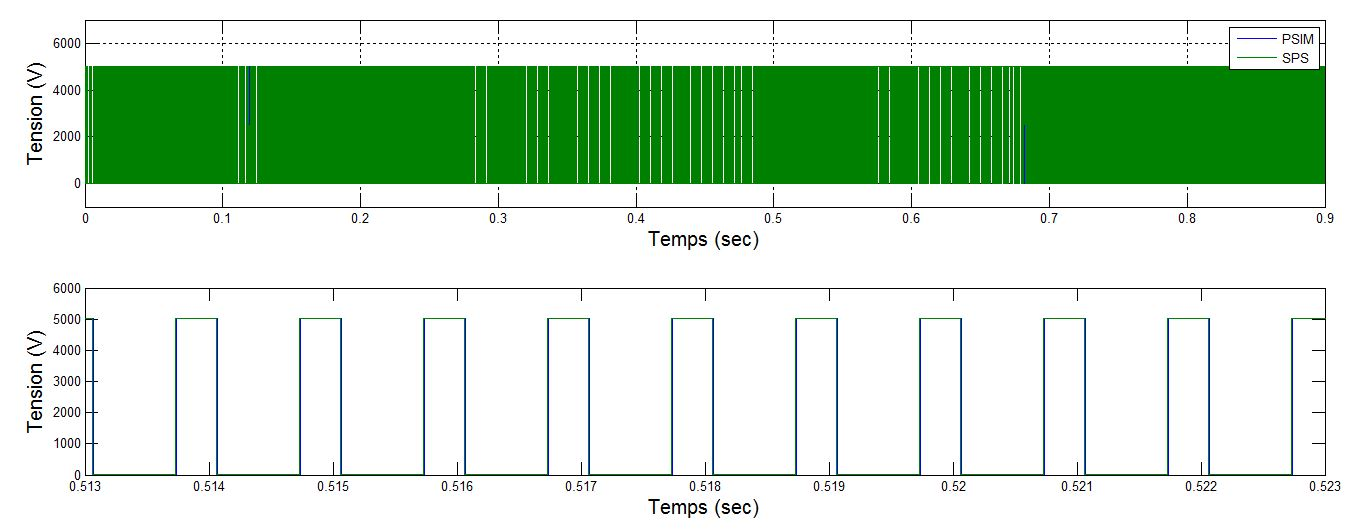
\includegraphics[scale=0.5]{Fig/Hacheur4Quadrants/HacheurTensionIGBT1u.jpg}
\caption{La tension au IGBT PSIM et SPS à un pas de calcul de 1us}
\label{hc_IG_ten_1}
\end{figure}

\begin{figure}[h!]
\centering
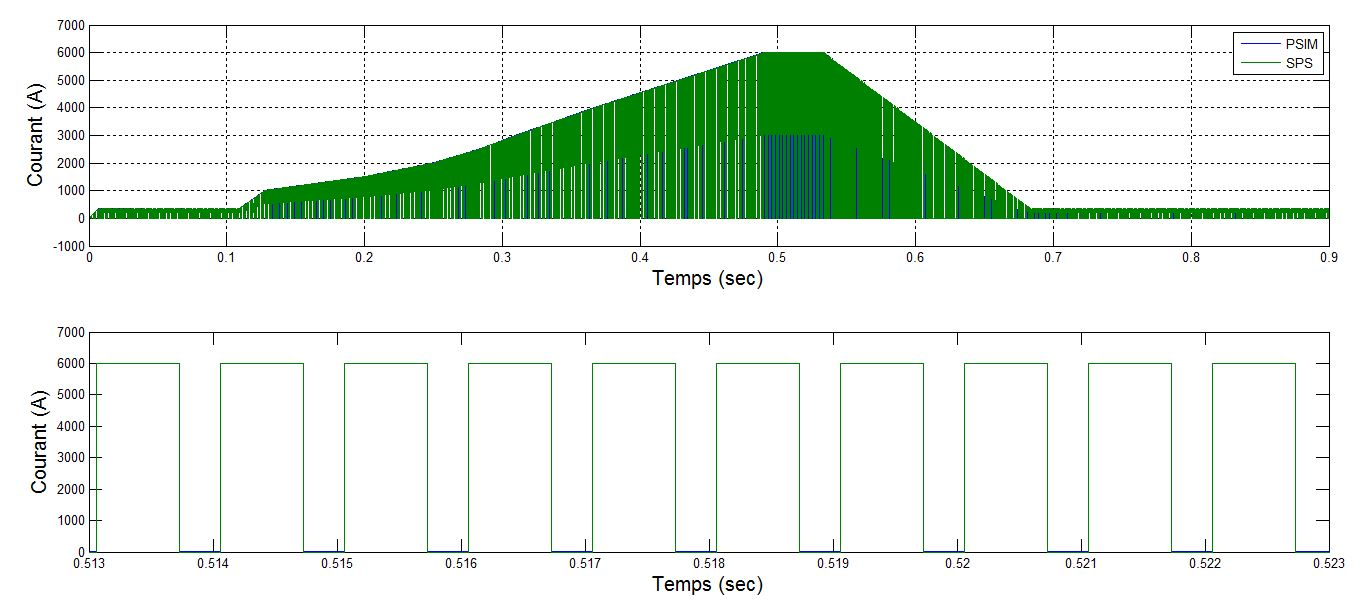
\includegraphics[scale=0.5]{Fig/Hacheur4Quadrants/HacheurCourantIGBT1u.jpg}
\caption{La tension au IGBT PSIM et SPS à un pas de calcul de 1us}
\label{hc_IG_cou_1}
\end{figure}
\clearpage

\subsection{DCP/DCN}

\subsubsection{Vérification à un pas de calcul de 50us}


\begin{figure}[h!]
\centering
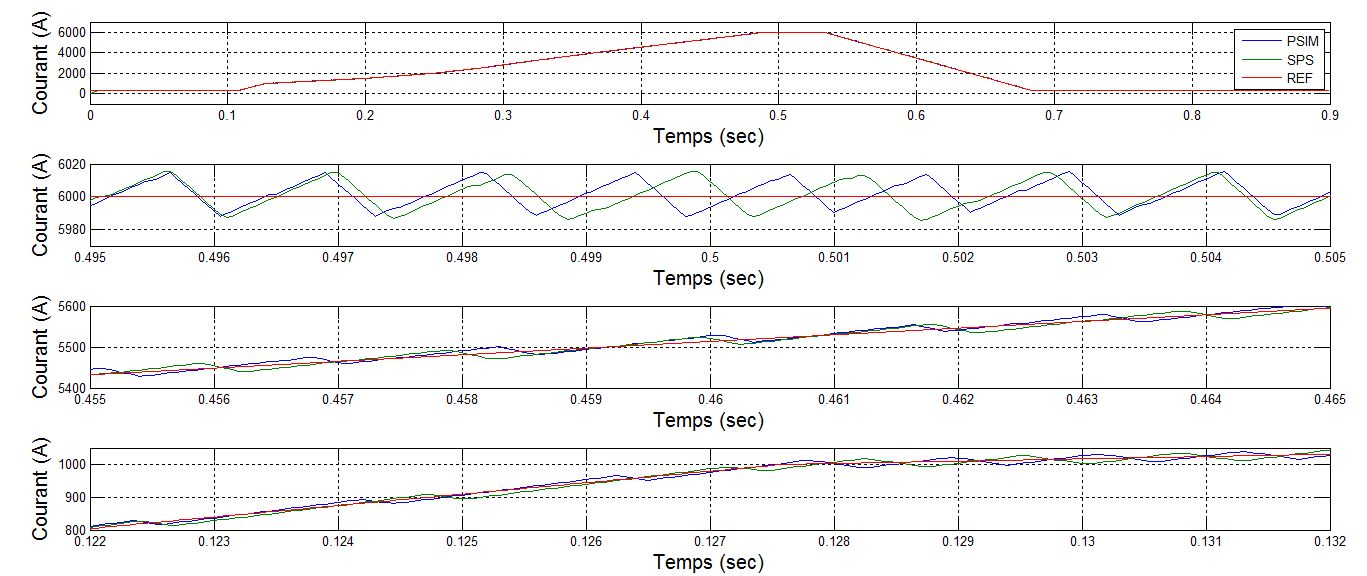
\includegraphics[scale=0.5]{Fig/DCPDCN/DCPCourantCharge50u.jpg}
\caption{Le courant sur la charge PSIM et SPS à un pas de calcul de 50us}
\label{DC_ch_cou_50}
\end{figure}


\begin{figure}[h!]
\centering
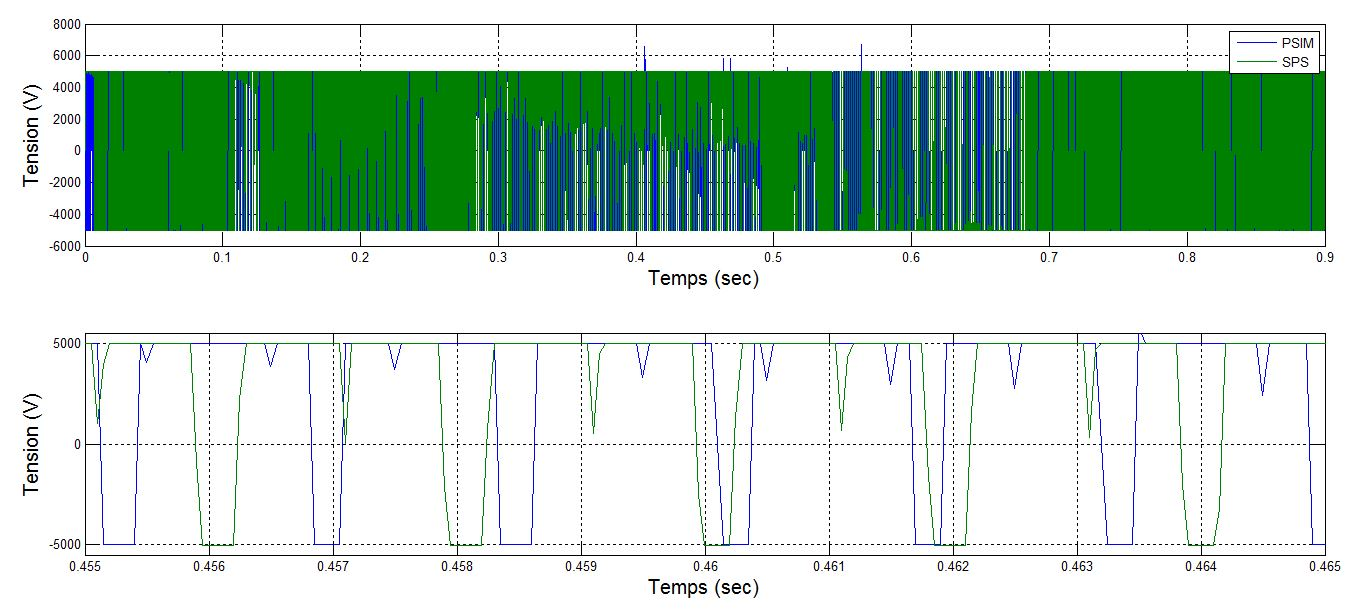
\includegraphics[scale=0.5]{Fig/DCPDCN/DCPTensionCharge50u.jpg}
\caption{La tension sur la charge PSIM et SPS à un pas de calcul de 50us}
\label{DC_ch_ten_50}
\end{figure}


\begin{figure}[h!]
\centering
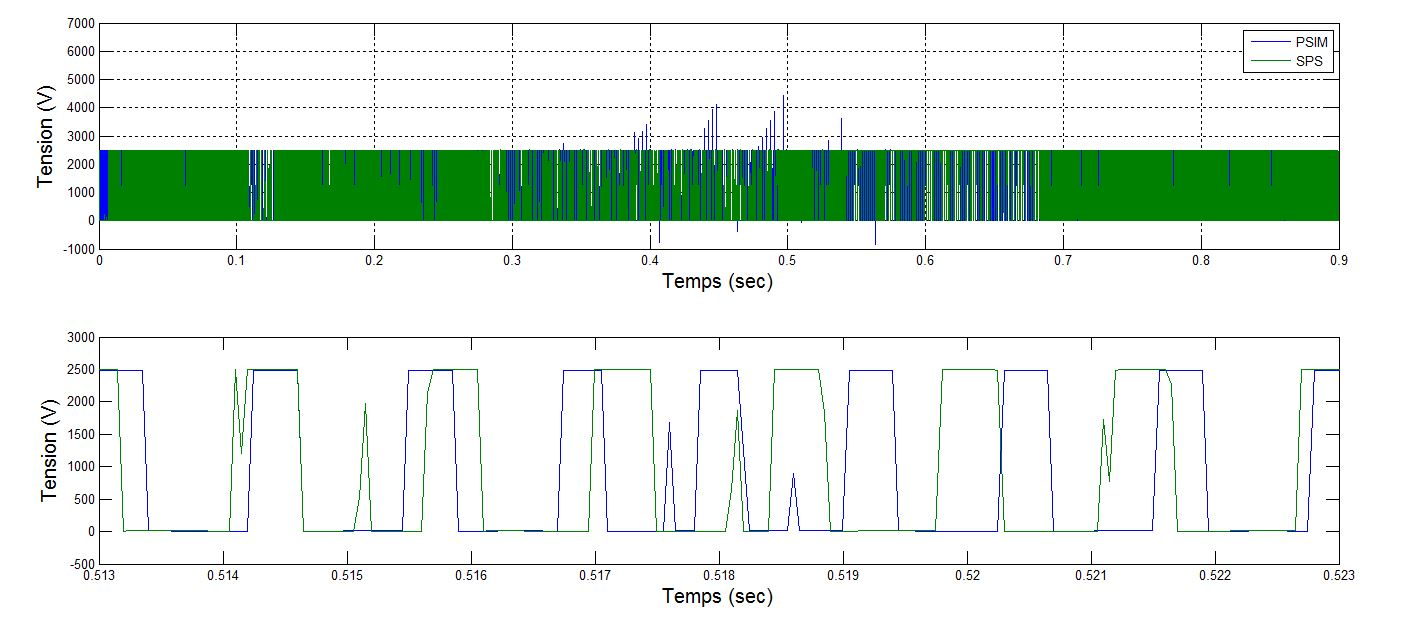
\includegraphics[scale=0.5]{Fig/DCPDCN/DCPTensionIGBT50u.jpg}
\caption{La tension au IGBT PSIM et SPS à un pas de calcul de 50us}
\label{DC_IG_ten_50}
\end{figure}

\begin{figure}[h!]
\centering
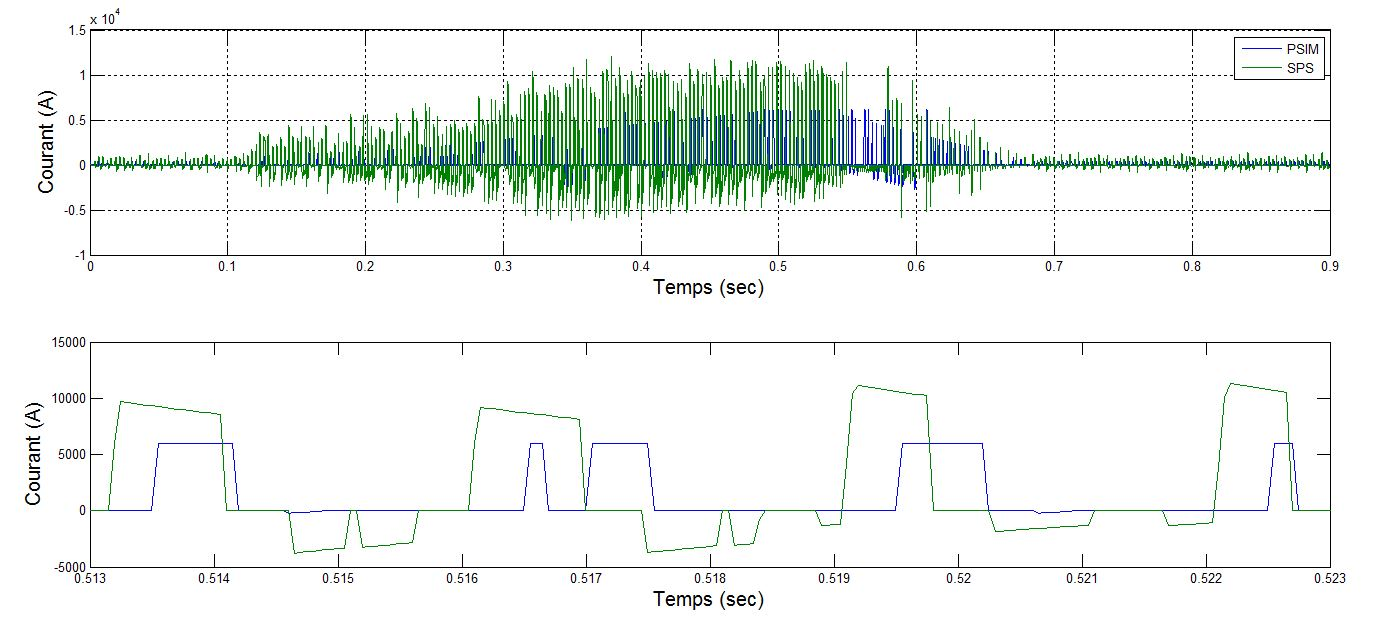
\includegraphics[scale=0.5]{Fig/DCPDCN/DCPCourantIGBT50u.jpg}
\caption{La tension au IGBT PSIM et SPS à un pas de calcul de 50us}
\label{DC_IG_cou_50}
\end{figure}
\clearpage

\subsubsection{Vérification à pas de calcul de 5us}

\begin{figure}[h!]
\centering
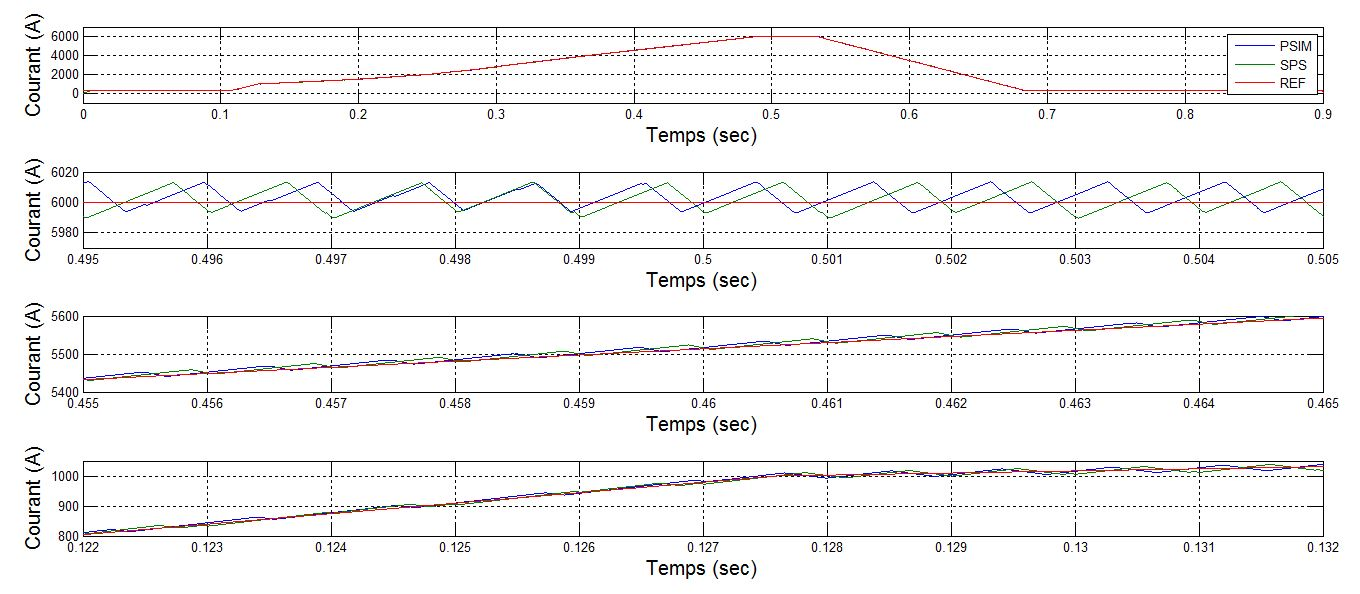
\includegraphics[scale=0.5]{Fig/DCPDCN/DCPCourantCharge5u.jpg}
\caption{Le courant sur la charge PSIM et SPS à un pas de calcul de 5us}
\label{DC_ch_cou_5}
\end{figure}


\begin{figure}[h!]
\centering
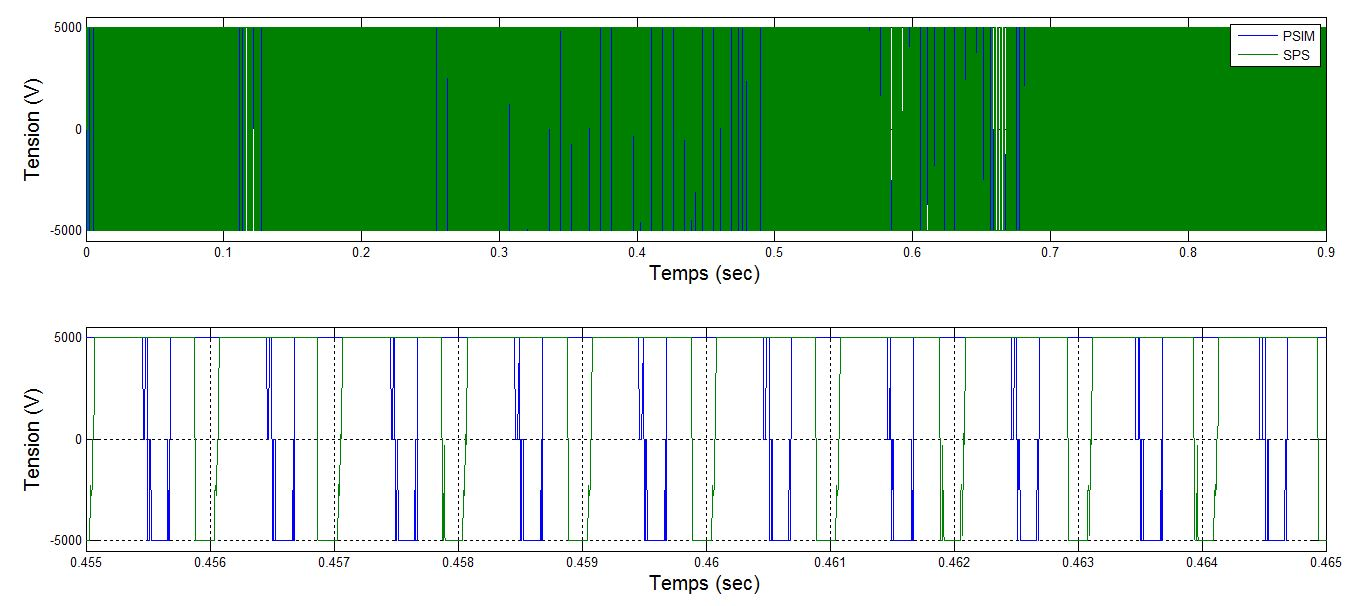
\includegraphics[scale=0.5]{Fig/DCPDCN/DCPTensionCharge5u.jpg}
\caption{La tension sur la charge PSIM et SPS à un pas de calcul de 5us}
\label{DC_ch_ten_5}
\end{figure}

\begin{figure}[h!]
\centering
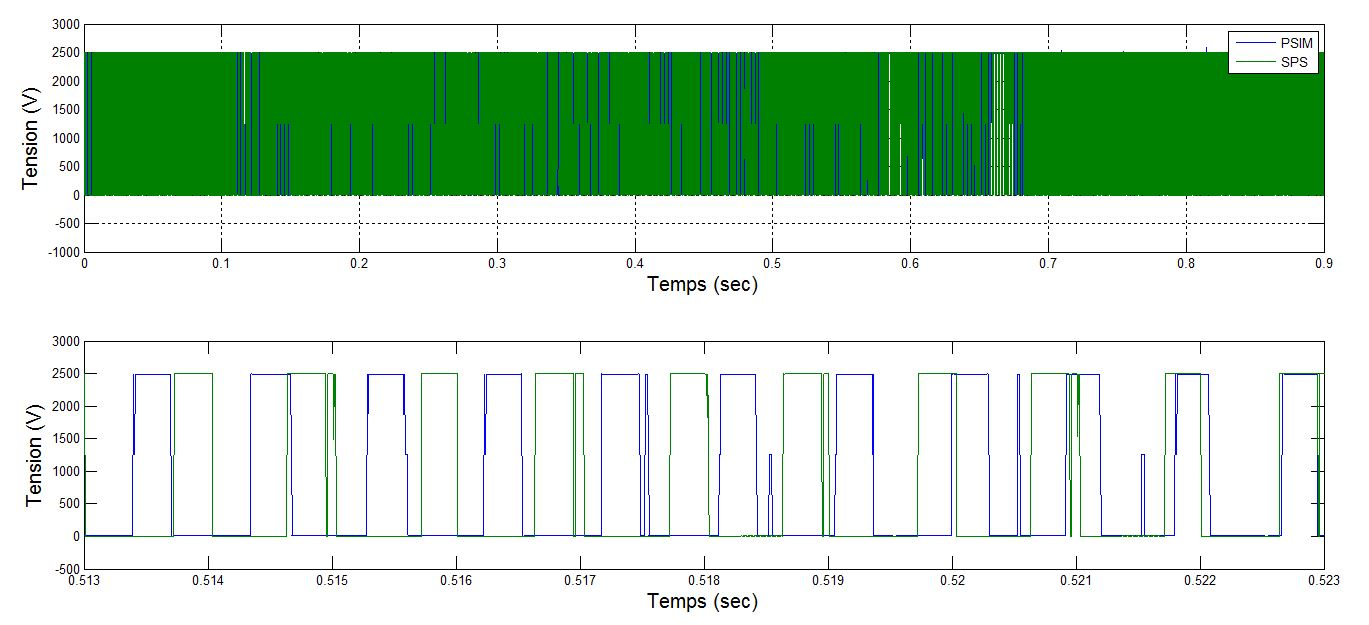
\includegraphics[scale=0.5]{Fig/DCPDCN/DCPTensionIGBT5u.jpg}
\caption{La tension au IGBT PSIM et SPS à un pas de calcul de 5us}
\label{DC_IG_ten_5}
\end{figure}

\begin{figure}[h!]
\centering
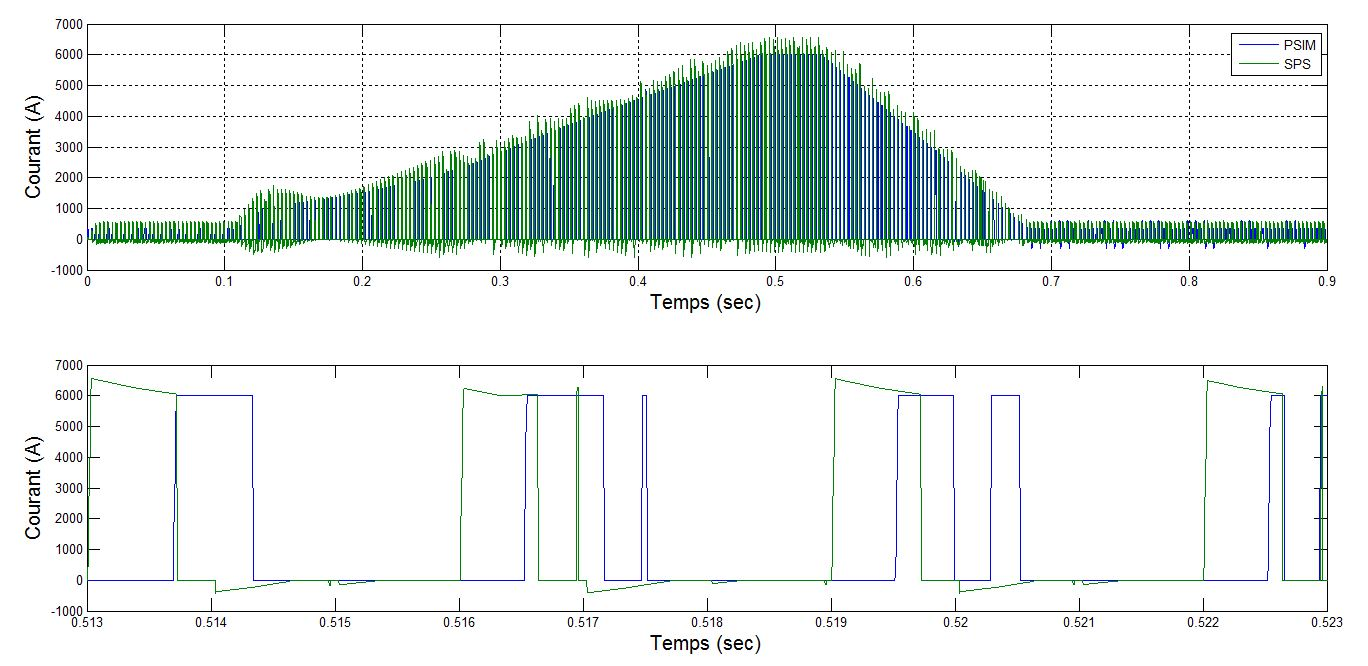
\includegraphics[scale=0.5]{Fig/DCPDCN/DCPCourantIGBT5u.jpg}
\caption{La tension au IGBT PSIM et SPS à un pas de calcul de 5us}
\label{DC_IG_cou_5}
\end{figure}


\clearpage
\subsubsection{Vérification à un pas de calcul de 1us}


\begin{figure}[h!]
\centering
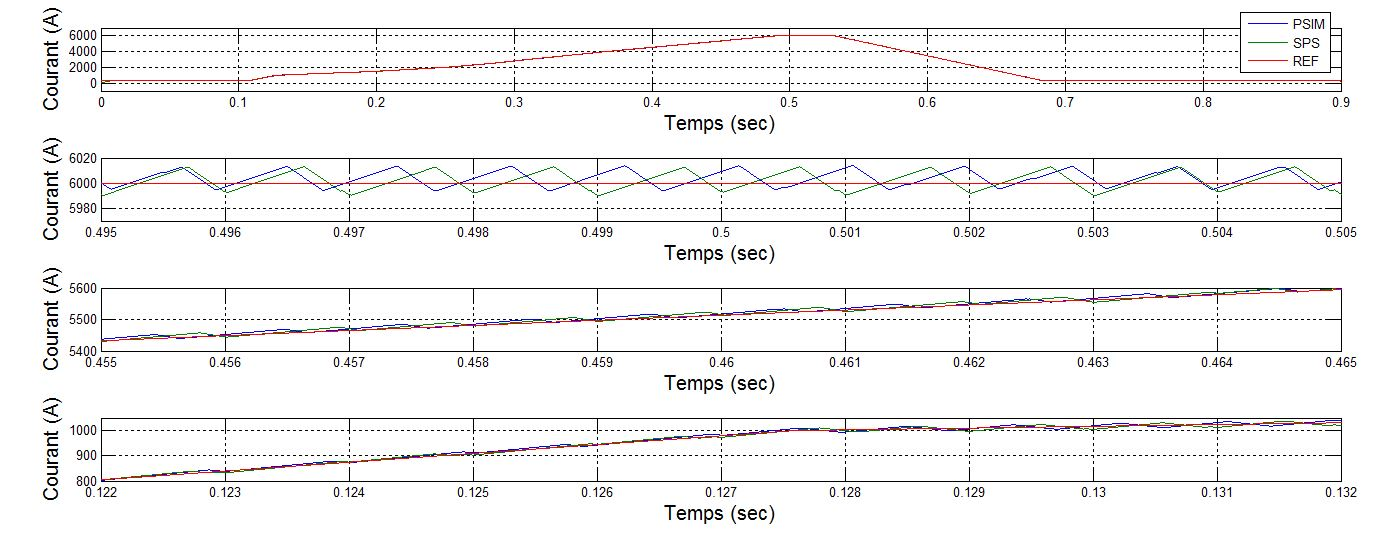
\includegraphics[scale=0.5]{Fig/DCPDCN/DCPCourantCharge1u.jpg}
\caption{Le courant sur la charge PSIM et SPS à un pas de calcul de 1us}
\label{DC_ch_cou_1}
\end{figure}


\begin{figure}[h!]
\centering
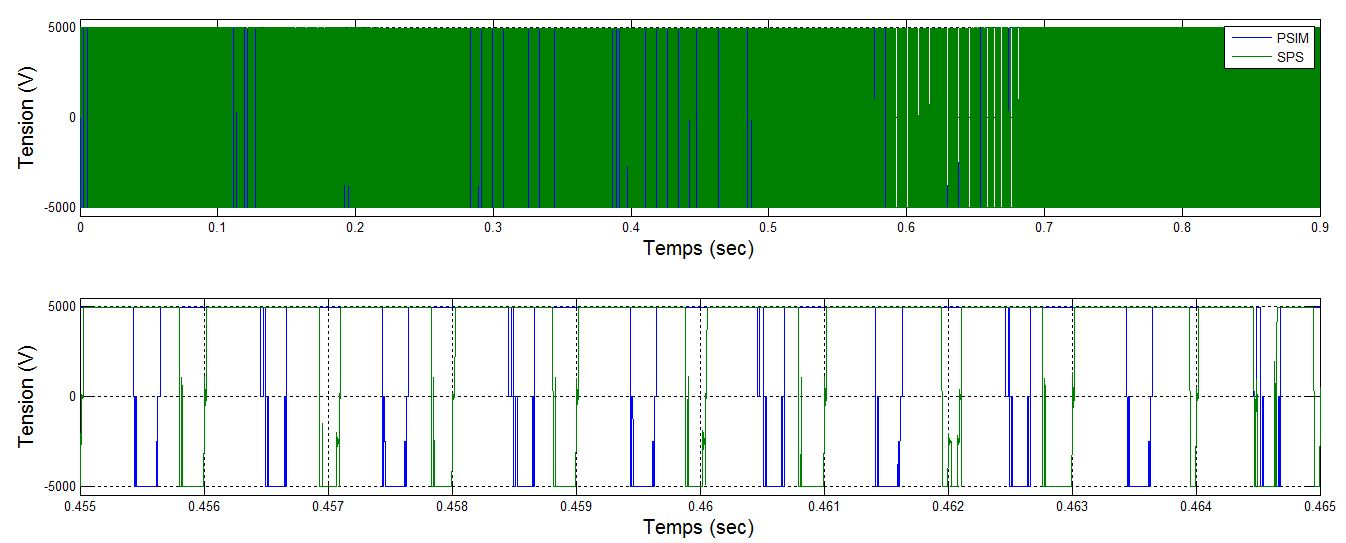
\includegraphics[scale=0.5]{Fig/DCPDCN/DCPTensionCharge1u.jpg}
\caption{La tension sur la charge PSIM et SPS à un pas de calcul de 1us}
\label{DC_ch_ten_1}
\end{figure}


\begin{figure}[h!]
\centering
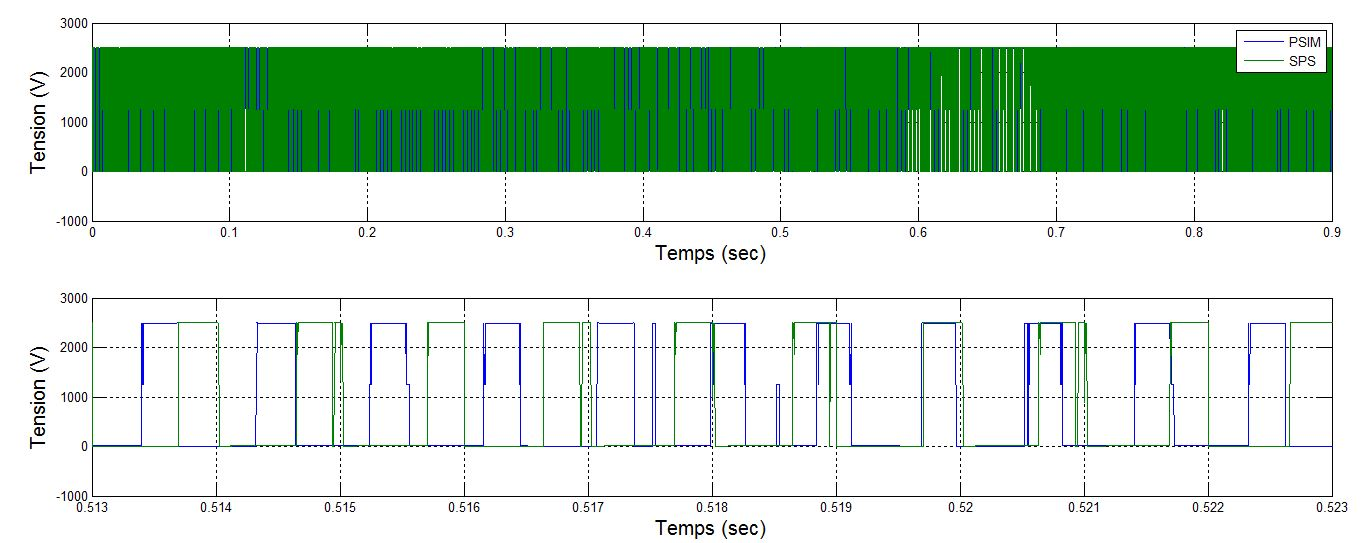
\includegraphics[scale=0.5]{Fig/DCPDCN/DCPTensionIGBT1u.jpg}
\caption{La tension au IGBT PSIM et SPS à un pas de calcul de 1us}
\label{DC_IG_ten_1}
\end{figure}

\begin{figure}[h!]
\centering
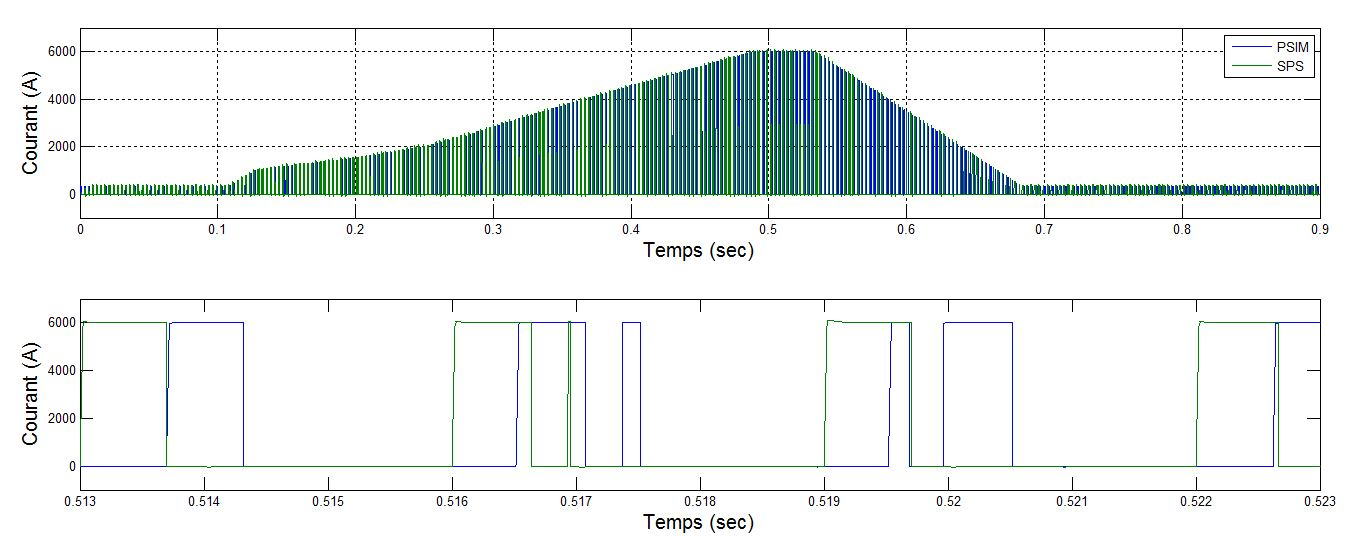
\includegraphics[scale=0.5]{Fig/DCPDCN/DCPCourantIGBT1u.jpg}
\caption{La tension au IGBT PSIM et SPS à un pas de calcul de 1us}
\label{DC_IG_cou_1}
\end{figure}





\end{document}